\documentclass[12pt, letterpaper]{article}
\usepackage[utf8]{inputenc}
\usepackage{amsmath}
\usepackage{amsthm}
\usepackage{colortbl}
\usepackage[a4paper, total={6.5in, 10in}]{geometry}

\usepackage{graphicx}
\graphicspath{ {/} }
\newtheorem{problem}{Problema}
\title{Computación Concurrente - Tarea 1}
\author{Damián Rivera González\\Alexis Hernandez Castro}

\begin{document}
\maketitle
\begin{itemize}
\item[1. ] Considera un problema computacional que puede resolverse secuencialmente en tiempo $n^3$, por ejemplo operaciones en matrices cuadradas $n\times n$ y la unidad de tiempo es 1 nanosegundo ($10^{-9}$). Des esta manera, si $n = 1000$, el cómputo tomaría $1000^3 \times 1 ns = 1s$. Supón que has creado un algoritmo concurrente que trabaja de manera completamente eficiente, es decir, el cómputo total tarda $\frac{n^3}{p}$ ($p$ es el número de hilos). Qué tan grande es la entrada que se puede manejar en: 

\begin{itemize}
\item[a, a) ] Un segundo y 8 hilos
$$\frac{n^3}{8} = 1s$$
$$n^3 = 1s \times 8$$
$$n = \sqrt[3]{1s \times 8}$$
$$n = 2000$$

\item[a, b) ] Un segundo y 1000 hilos
$$\frac{n^3}{1000} = 1s$$
$$n^3 = 1s \times 1000$$
$$n = \sqrt[3]{1s \times 1000}$$
$$n = 10000$$

\item[a, c) ] Un segundo y 1000000 hilos
$$\frac{n^3}{1000000} = 1s$$
$$n^3 = 1s \times 1000000$$
$$n = \sqrt[3]{1s \times 1000000}$$
$$n = 100000$$

\item[b, a) ] Un minuto y 8 hilos
$$\frac{n^3}{8} = 60s$$
$$n^3 = 60s \times 8$$
$$n = \sqrt[3]{60s \times 8}$$
$$n = 7829.73$$

\item[b, b) ] Un minuto y 1000 hilos
$$\frac{n^3}{1000} = 60s$$
$$n^3 = 60s \times 1000$$
$$n = \sqrt[3]{60s \times 1000}$$
$$n = 39148.67$$

\item[b, c) ] Un minuto y 1000000 hilos
$$\frac{n^3}{1000000} = 60s$$
$$n^3 = 60s \times 1000000$$
$$n = \sqrt[3]{60s \times 1000000}$$
$$n = 391486.76$$

\item[c, a) ] Un mes y 8 hilos
$$\frac{n^3}{8} = 2592000s$$
$$n^3 = 2592000s \times 8$$
$$n = \sqrt[3]{2592000s \times 8}$$
$$n = 274731.41$$

\item[c, b) ] Un mes y 1000 hilos
$$\frac{n^3}{1000} = 2592000s$$
$$n^3 = 2592000s \times 1000$$
$$n = \sqrt[3]{2592000s \times 1000}$$
$$n = 1373657.09$$

\item[c, c) ] Un mes y 1000000 hilos
$$\frac{n^3}{1000000} = 2592000s$$
$$n^3 = 2592000s \times 1000000$$
$$n = \sqrt[3]{2592000s \times 1000000}$$
$$n = 13736570.91$$
\end{itemize}
¿Cuántos hilos se necesitan si se quisiera resolver un problema con $n = 10^6$ en un año? 

$$\frac{(10^6)^3}{p} = 31536000s$$
Despejando a $p$ tenemos:
$$p = \frac{1\times 10^{18}}{31536000s} = 31709791983\leftarrow hilos$$


\item[5. ] Considera la siguiente clase que representa un contador:\\
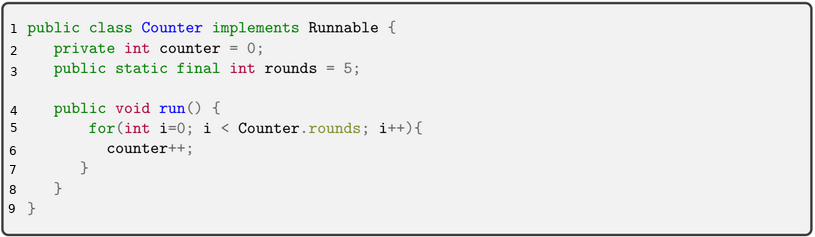
\includegraphics[width=\textwidth]{Codigo5}\\
Suponiendo que los hilos se ejecutan concurrentemente sobre el contador. Contesta las siguientes preguntas.
\begin{itemize}
\item[a) ] Demuestra que no existe una ejecución en donde el valor del contador sea 0.\\

Como sabemos, hay dos hilos, llamemosle $h1$ y $h2$, para los cuales sin importar cuantas iteraciones tengan en su ciclo $for$, la última instrucción que se lleva a cabo es $counter++$, por lo que al menos uno de los dos hilos, $h1$ o $h2$, terminará su ejecución con esta instrucción, y si en un inicio $counter = 0$, al final su valor será aumentado en una unidad. Por lo tanto el valor de $counter$ no puede terminar con valor 0. 

\item[b) ] Demuestra que no existe una ejecución en donde el valor del contador sea 1.

[Por contradicción] Sabemos que hay dos hilos, llamemosle $h1$ y $h2$. Supongamos que el valor del contador termina en 1. Como sabemos que cada hilo ejecuta el método $run$ en el cual la última instrucción es $counter++$, supongamos sin perdida de generalidad que el hilo $h2$ termina la útlima ejecución de $counter++$ significa que el $h2$ leyó $counter = 0$ teniendo así dos casos: 
\begin{itemize}
\item[Caso 1. ] Es la última iteración del $for$ en $h2$.\\
Lo cual implica que $h2$ leyó 5 veces a $counter = 0$, lo cual no se podría puesto que $h1$ ha terminado con todas sus iteraciones y al menos aumento en una unidad el valor de $counter$, por lo tanto $h2$ no pudo haber leido $counter = 0$.

\item[Caso 2. ] No es la última iteración del $for$ en $h2$.\\
Lo que significa que al menos $h2$ o $h1$ aumentaran en una unidad el valor de $counter$ por lo que $h2$ no podría terminar leyendo en la penúlitma acción a $counter = 0$.
\end{itemize} 

\item[c) ] Muestra una ejecución en donde el valor final del contador sea 2.\\
\resizebox*{.75\textwidth}{!}{
\begin{tabular}{|c | c | c|}
\hline
\rowcolor[gray]{0.9}$H1$ & $H2$ & Memoria \\
\hline 
PC 4 & PC 4 & counter = 0\\
PC 5, i = 0 & PC 5, i = 0 & counter = 0\\
PC 6, i = 0, read(counter)& PC 6, i = 0, read(counter) = 0 & counter = 0\\
PC 6, i = 1, write(counter++) & & counter = 1\\
PC 6, i = 1, read(counter)& & counter = 1\\
PC 6, i = 2, write(counter++) & & counter = 2\\
PC 6, i = 2, read(counter)& & counter = 2\\
PC 6, i = 3, write(counter++) & & counter = 3\\
PC 6, i = 3, read(counter)& & counter = 3\\
PC 6, i = 4, write(counter++)& & counter = 4\\
 & PC 6, i = 1, write(counter++) & counter = 1\\
PC 6, i = 4, read(counter)& PC 6, i = 1, read(counter) & counter = 1\\
 & PC 6, i = 2, write(counter++) & counter = 2\\
 & PC 6, i = 2, read(counter) & counter = 2\\
 & PC 6, i = 3, write(counter++) & counter = 3\\
 & PC 6, i = 3, read(counter) & counter = 3\\
 & PC 6, i = 4, write(counter++) & counter = 4\\
 & PC 6, i = 4, read(counter) & counter = 4\\
 & PC 6, i = 5, write(counter++) & counter = 5\\ 
PC 6, i = 5, write(counter++) & & counter = 2\\
\hline
\end{tabular}}\\

\item[d) ] Muestra una ejecución en donde el valor final del contador sea 7.\\
\resizebox*{.75\textwidth}{!}{
\begin{tabular}{|c | c | c|}
\hline
\rowcolor[gray]{0.9}$H1$ & $H2$ & Memoria \\
\hline 
PC 4 & PC 4 & counter = 0\\
PC 5, i = 0 & PC 5, i = 0 & counter = 0\\
PC 6, i = 0, read(counter)& PC 6, i = 0, read(counter) = 0 & counter = 0\\
PC 6, i = 1, write(counter++) & PC 6, i = 1, write(counter++) & counter = 1\\
PC 6, i = 1, read(counter)& PC 6, i = 1, read(counter) & counter = 1\\
PC 6, i = 2, write(counter++) & PC 6, i = 2, write(counter++) & counter = 2\\
PC 6, i = 2, read(counter)& & counter = 2\\
PC 6, i = 3, write(counter++) & & counter = 3\\
PC 6, i = 3, read(counter)& & counter = 3\\

PC 6, i = 4, write(counter++) & & counter = 4\\
PC 6, i = 4, read(counter)& PC 6, i = 2, read(counter) & counter = 4\\
PC 6, i = 5, write(counter++) & PC 6, i = 3, write(counter++) & counter = 5\\
 & PC 6, i = 3, read(counter) & counter = 5\\
 & PC 6, i = 4, write(counter++) & counter = 6\\
 & PC 6, i = 4, read(counter) & counter = 6\\
 & PC 6, i = 5, write(counter++) & counter = 7\\

\hline
\end{tabular}}\\


\end{itemize}



\item[7. ] Propón un algoritmo de exclusión mutua para 3 hilos basado en turnos round robin.

\begin{itemize}
\item[a) ] Demuestra que cumple con la propiedad de exclusión.

\item[b) ] ¿Es libre de deadlock?

\item[c) ] ¿Es libre de hambruna?
\end{itemize}



\item[8. ] Eres uno de los $P$ prisioneros arrestados recientemente, pero el guardia de la carcel quiere darles una oportunidad para salvarse. Él ordenará a todos los prisioneros en una línea, y colocará sombreros de color rojo o azul en sus cabezas. Ningún prisionero conoce el color de su propio sombrero o el color de cualquier sombrero detrás de él, pero si puede ver los sombreros de los prisisoneros que están en frente. El guardia comenzará desde el final de la línea y pregunta a cada prisionero el color de su propio sombrero, el cual solo puede responder rojo o azul. Si da con la respuesta incorrecta será aventado a los cocodrilos, pero si contesta corrrectamente será liberado. Cada preso puede escuchar la respuesta de los prisioneros detrás de él, pero no puede decir si ese prisionero tenía razón o no.

\begin{itemize}
\item[a) ] Diseña una estrategía para salvar al menos a $P-1$ prisioneros.
Como sabemos que solo hay dos colores $Rojo$ y $Azul$, los prisioneros se pondrán de acuerdo para elegir un color y dar la clave sobre este. Supongamos que eligen el color $Rojo$. Entonces el primer prisionero que responde (el de hasta atrás) verá la cantidad de sombreros rojos, si el número de sombreros rojos es par, el prisionero responderá $"Rojo"$, si el color de sombreros rojos es impar entonces el prisionero responderá $"Azul"$, entonces todos sabrán desde un inicio si el número de sombreros rojos es par o impar. Supongamos que el último prisionero dice $Rojo$, entonces sabrán que hay un número par de sombreros rojos. Para los primeros que vean un número par de sombreros rojos sin haber escuchado previamente que alguien respondierá rojo, entonces sabrán que su sombrero es azul, el primer prisionero que vea una cantidad impar de sombreros sabrá que su sombrero es rojo, pues el hace la cantidad par de sombreros. Después de él, todos sabrán que ya hay una cantidad impar de sombreros rojos, por lo que todos los siguientes que vean una cantidad impar sabrán que tienen un sombrero azul, el primero que vea una cantidad par de sombreros sabrá que el tiene el sombrero rojo que hace la cantidad par. Y así sucecivamente.

Ahora, si desde un inicio el primer prisionero dice $"Azul"$, sabrán todos que hay una cantidad impar de sobreros rojos, por lo que el primero que vea una cantidad par de sombreros, sabrá que su sombrero es el que forma la cantidad par, cambiando ahora la cantidad de rojos a par, y todos los que vean una cantidad par o impar según la cantidad actual que hay de sombreros rojos sabrán que tienen un sombrero azul. Y así sucesivamente.

Por lo que deben fijar un color desde el principio, y dirán si el color fijado si el primer prisionero ve una cantidad par de este o el color contrario si ve una cantidad impar del color fijado.
\item[b) ] Supón que ahora el guardia puede utilizar k colores. ¿Cuál sería ahora la estrategia?
\end{itemize}


\end{itemize}



\end{document}